\newpage
\hypertarget{common cspConstraint}{}
\subsection{Implementing SetDefaultNumber}
\genHeader

\begin{itemize}

\item[$\blacktriangleright$]  Navigate and expand ``DictionaryCodeAdapter/src/csp.constraints.'' Open \texttt{SetDefaultNumber.java} and edit this file until it
matches Fig.~\ref{eclipse:setDefaultImpl}.

\vspace{0.5cm}

\begin{figure}[htbp]
\begin{center}
  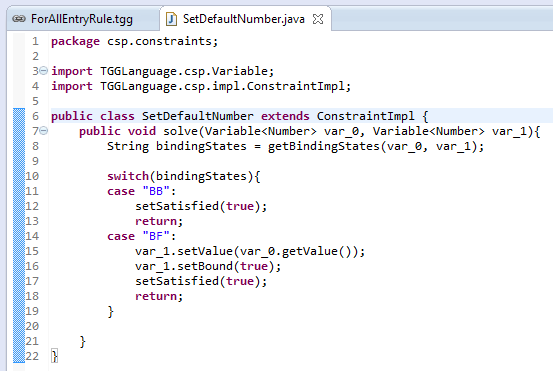
\includegraphics[width=0.9\textwidth]{eclipse_setDefaultNumberImplementation}
  \caption{Completing the custom \texttt{setDefaultNumber} constraint}
  \label{eclipse:setDefaultImpl}
\end{center}
\end{figure}

\item[$\blacktriangleright$] After saving, and run \texttt{TGGMain} one more time. The initial and final \texttt{tree} variants should now be nearly
identical! The only difference should be that, instead of each \texttt{entry.index} value increasing (as seen in \texttt{tree.xmi}), each value should now be
set to exactly 2. Their order may be different, depending on how the transformation processed them, but their \texttt{index} values should all  be correct.

\vspace{0.5cm}

\item[$\blacktriangleright$] Your transformation is nearly complete! The only remaining step is to unparse this final tree structure into an output filesystem.
Before we move on however, let's reflect on how easy and short it was to implement this `backwards' transformation. If we were to use another method (such as
SDMs), we would have had to create at least six more independent rules to handle this. Instead, TGGs gave us this direction for free!

\end{itemize}
